\chapter{Project Schedule}
In this section the project schedule is shown. It has been implemented from a Gantt chart, attached on the next page.

This project is focused in developing a complete space sensor platform with an on ground post-processing interface. For that reason on the project schedule tu critical path are observed. 

First one, corresponds to project management, administrative and communication tasks. These tasks are all project duration tasks, because if one of these tasks stops all project is affected. These tasks are essential to coordinate and to carry out the project.

Second critical path, is related with the development of the sensor platform and is not as easy to see as the first one. The whole project is been structured with fix date milestones in order to control deadlines and progress. Therefore, even a complete critical path (marked in red) at a first sight is not seen, it rally exists. Because every milestone have a fixed finishing date, any task expected to end before the milestone that is delayed, means that the whole project is affected. All tasks are connected through the milestones, so taking this fact into account, now is possible to see the critical path on the sensor development tasks.

Also, sensor development has been divided in three parts: investigation and creation of the sensors, development of a modular module to include all the sensors and a data on-ground post-processing interface to interpret the sensors information. With this development scheme on mind, is it possible to appreciate how technology development tasks succeed each other in groups of three. For example, firstly sensors are build, a short period after the modular case starts its production and a little more after the interface also starts. When the sensors task end, automatically starts the sensors testing task while the previous two ones still in progress. This is how principally the tasks succeed between them.

\begin{landscape}
	\begin{figure}[H]
	\centering
	\begin{tabular}{@{}c@{\hspace{.5cm}}c@{}}
		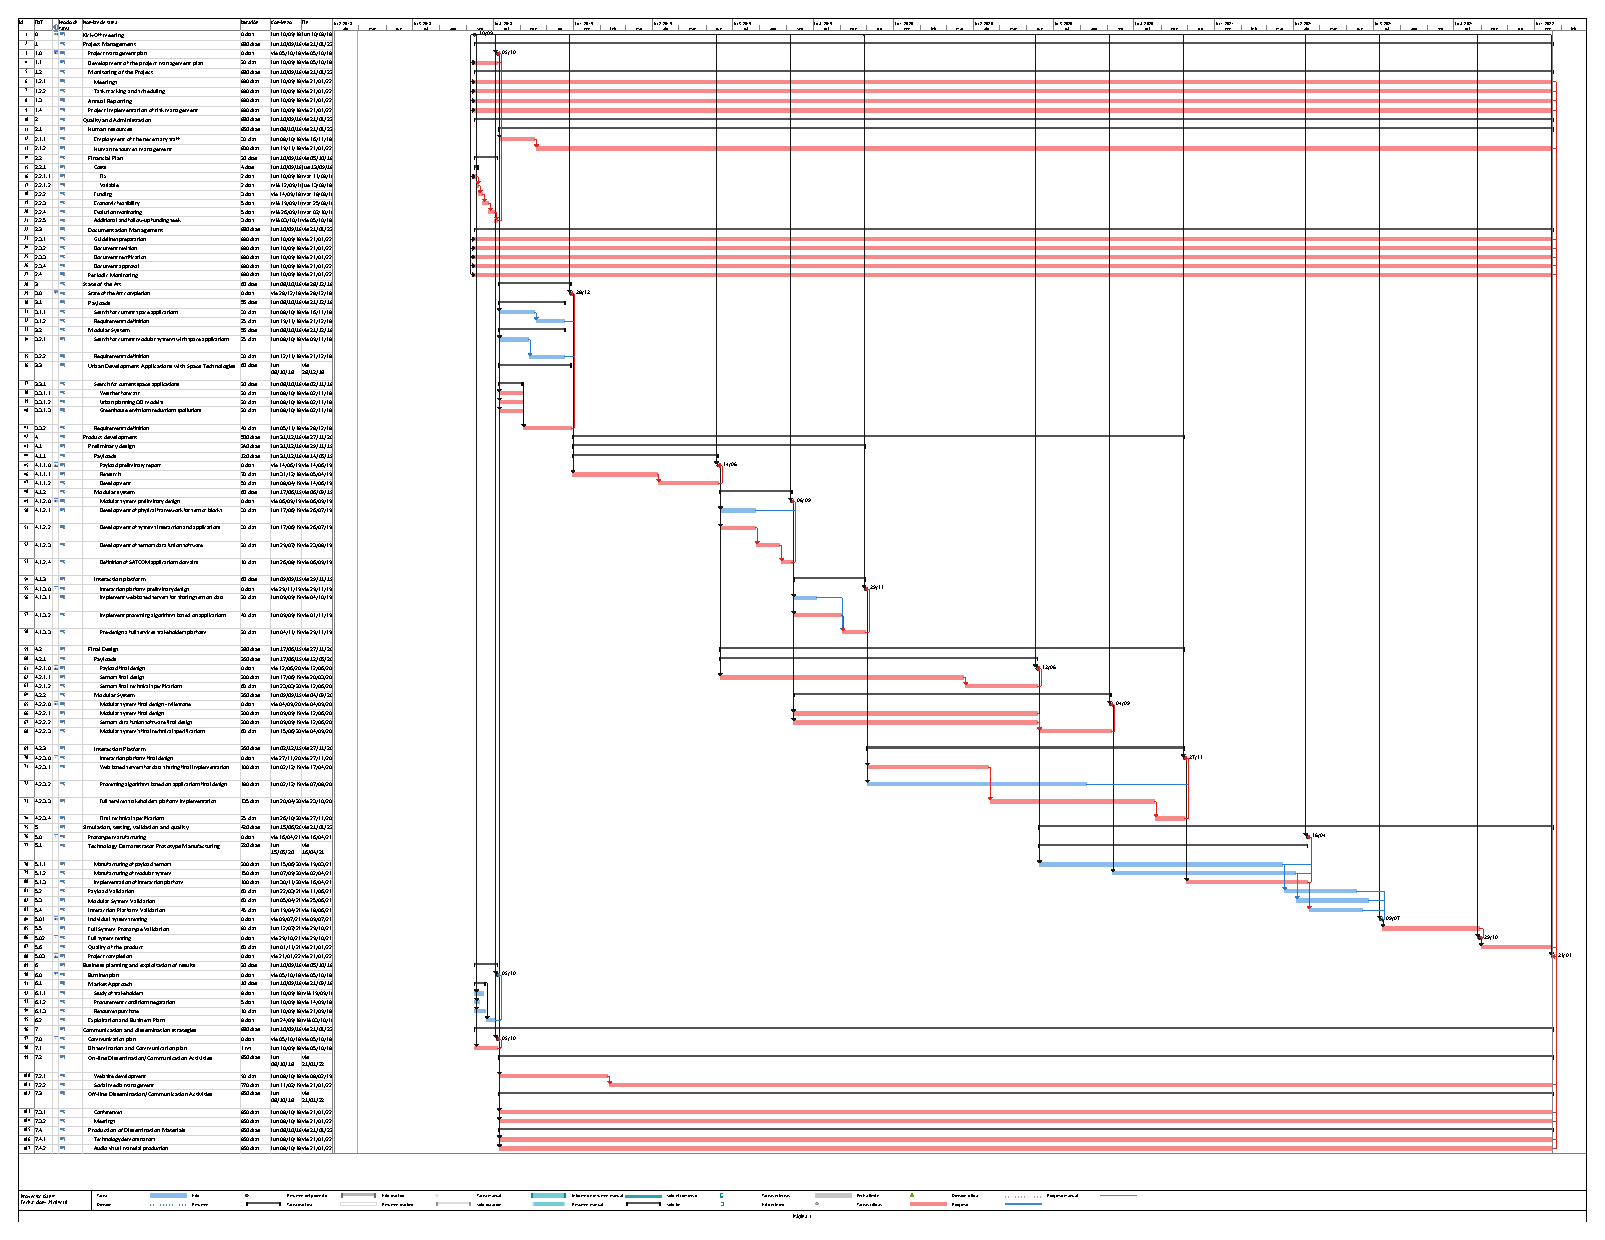
\includegraphics[page=1,width=1.2\textwidth]{./images/gantt/GANTT.pdf}
	\end{tabular}
	\caption{Gantt chart}
	\label{Gantt}
	\end{figure}
\end{landscape}